% === Begin Label Data ===
% ID: 806
% 难度星级: 
% 标签: 
% 备注: 
% 组卷引用次数: 0
% === End  Label Data ===

\begin{problem}{2018}{G}{全国I卷}{9}{函数}
已知函数 $ f(x)=\begin{cases} e^x, & x\leqslant 0, \\ \ln x, & x>0. \end{cases} $，$ g(x)=f(x)+x+a $.若 $ g(x) $ 存在 2 个零点，则 $ a $ 的取值范围是 (\hspace{1cm})
\begin{choices}
\choice{{${[-1,0)}$}}
\choice{{${[0,+\infty)}$}}
\choice{{${[-1,+\infty)}$}}
\choice{{${[1,+\infty)}$}}
\end{choices}
\end{problem}

\begin{answer}
C
\end{answer}

\begin{solutions}
思路 1：首先作出 $ y=f(x) $ 的图像与直线 $ y=-x-a $ 的图像，如图所示。  
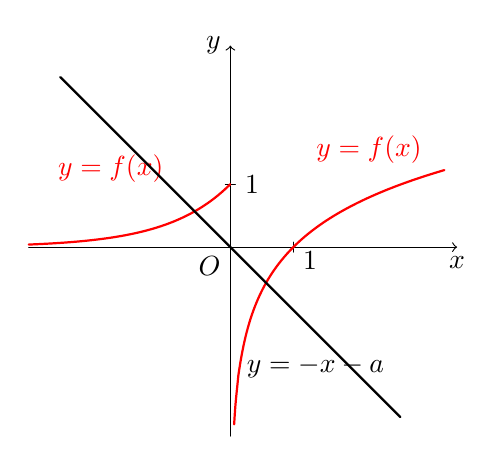
\begin{tikzpicture}[line cap=round,line join=round,scale=0.8]
\usetikzlibrary{calc}

% --- axes ---
\draw[->] (-3.2,0) -- (3.6,0) node[below] {$x$};
\draw[->] (0,-3.0) -- (0,3.2) node[left] {$y$};
\node[below left] at (0,0) {$O$};

% ticks/labels (match the sketch: mark y=1 and x=1)
\draw (-0.08,1) -- (0.08,1) node[right] {$1$};
\draw (1,-0.08) -- (1,0.08) node[below right] {$1$};

% --- red piecewise f(x): e^x (x<=0) and ln x (x>0) ---
\draw[red,thick,smooth,samples=160,domain=-3.2:0]
  plot (\x,{exp(\x)});
\draw[red,thick,smooth,samples=200,domain=0.06:3.4]
  plot (\x,{ln(\x)});

\node[red] at (-1.9,1.25) {$y=f(x)$};
\node[red] at (2.2,1.55) {$y=f(x)$};

% --- line y = -x - a (take a=0 for the picture-style schematic) ---
% so the line crosses (0,0) and has slope -1
\draw[thick] (-2.7,2.7) -- (2.7,-2.7);
\node at (1.35,-1.9) {$y=-x-a$};

\end{tikzpicture}

显然，当且仅当 $ -a\leqslant 1 $，即 $ a\geqslant -1 $ 时，$ f(x) $ 的图像与直线 $ y=-x-a $ 有两个交点，故当且仅当 $ a\geqslant -1 $ 时，$ g(x) $ 存在两个零点，故选 C。

思路 2：写出 $ g(x) $ 的分段式。  
$$
g(x)=\begin{cases}
e^x+x+a, & x\leqslant 0, \\
\ln x+x+a, & x>0.
\end{cases}
$$  
当 $ x\leqslant 0 $ 时，$ g(x)=e^x+x+a $ 在 $ (-\infty,0] $ 为增函数。  
又 $ g(0)=a+1 $.  
若 $ a+1<0 $，即 $ a<-1 $，有 $ g(x)\leqslant g(0)<0 $，这时 $ g(x) $ 在 $ (-\infty,0] $ 无零点。  
若 $ a+1\geqslant 0 $，即 $ a\geqslant -1 $，有 $ g(0)\geqslant 0 $，$ g(-1-a)=e^{-(1+a)}-1\leqslant 0 $，这时 $ g(x) $ 在 $ (-\infty,0] $ 有一个零点.  
故当且仅当 $ a\geqslant -1 $ 时，$ g(x) $ 在 $ (-\infty,0] $ 有一个零点.  

当 $ x>0 $ 时，$ g(x)=\ln x+x+a $ 在 $ (0,+\infty) $ 为增函数.  
又 $ g(e^{-a})=e^{-a}>0 $，$ g(1)=a+1 $.  
若 $ a+1<0 $，即 $ a<-1 $，有 $ g(1)<0 $，这时 $ g(x) $ 有一个零点.  
若 $ a+1\geqslant 0 $，即 $ a\geqslant -1 $，有 $ g(e^{-(1+a)})=e^{-(1+a)}-1\leqslant 0 $，这时 $ g(x) $ 有一个零点.  
故对 $ a $ 的任何取值，$ g(x) $ 在 $ (0,+\infty) $ 有一个零点.  

综上，当且仅当 $ a\geqslant -1 $ 时，$ g(x) $ 有两个零点. 故选 C.
\end{solutions}